\section{Introduction}

With the recent development of computational journalism \cite{Cohen2011, Hassan15}, on-line fact-checkers such as FactCheck\footnote{ {\scriptsize\url{http://www.factcheck.org}}}, Snopes\footnote{{\scriptsize\url{http://www.snopes.com}}}, PolitiFact\footnote{{\scriptsize \url{http://www.politifact.com}}}, TruthorFiction\footnote{{\scriptsize\url{http://www.truthorfiction.com}}} or OpenSecrets\footnote{{\scriptsize \url{http://www.opensecrets.org}}}, and ClaimBuster\footnote{{\scriptsize\url{http://idir-server2.uta.edu/claimbuster}}} have lately gained unprecedented attention as their goal is to verify on-line information for  public opinion and automate Web-scale fact-checking.
But estimating the veracity of data still remains  a  challenging problem: extracting structured information from large, heterogeneous corpora of textual and multimedia documents, and  integrating these  multi-source data are difficult tasks. Web  data and micro-texts from social media can be noisy, outdated, incorrect, conflicting, and thus unreliable, often due to information extraction errors, disagreements, biased observations, disparate or low quality of the sources. 
 
 Many truth discovery methods have been proposed to deal with data veracity estimation (see \cite{Berti2015} for a survey). They are mostly applied to structured data and compute iteratively the accuracy of the sources claiming some data as a function of the veracity scores of their data and the veracity scores are computed as a function of the accuracy of their sources. Recent approaches have been developed to discover true values extracted from textual content in a large corpus of Web sources using various information extractors \cite{Dong2014,YuHCJWZHVM14}.  
These solutions extend previous probabilistic models based on iterative vote counting and integrate the extraction systems' error in truth discovery computation.
 
 Nevertheless, most approaches operate on a static set of structured claims from a fixed corpus of information sources. They usually do not expand dynamically the search space to gather additional evidences and controversial or corroborating claims. Moreover, several studies have proven that a ``one-fits-all'' solution does not seem to be achievable for a wide range of truth discovery scenarios \cite{Wagui14} and we argue that ensembling truth discovery methods can significantly improve the quality performance of current results \cite{BigData15}.
 
In this demo, we present $\VERA$, a Web-based platform that supports the pipeline of truth discovery from Web unstructured corpus and tweets: ranging from information extraction from raw texts and micro-texts and data fusion to truth discovery and visualization. $\VERA$ offers several advantages over previous work as it includes: 
\renewcommand{\labelitemi}{$-$}
\begin{itemize}
\item Extraction and fusion of multi-source information to answer a factual query defined by the user;
\item Combination of multiple truth discovery algorithms using  ensembling in order to effectively discover true values from conflicting ones;
\item Explanation of the truth discovery results;
\item Visualization artifacts to better understand the information space with disagreeing vs. agreeing sources and corroborating vs. conflicting claims.
\end{itemize}


 To the best of our knowledge, this work is the first attempt to demonstrate truth discovery in action from Web data and Twitter data, overcoming limitations of single truth discovery methods with ensembling to estimate data veracity. $\VERA$ platform, RESTful API, and additional material including real-world datasets and a synthetic dataset generator are available at:  {\url{http://da.qcri.org/dafna/}}.


\begin{figure}[t]
 \begin{center}
  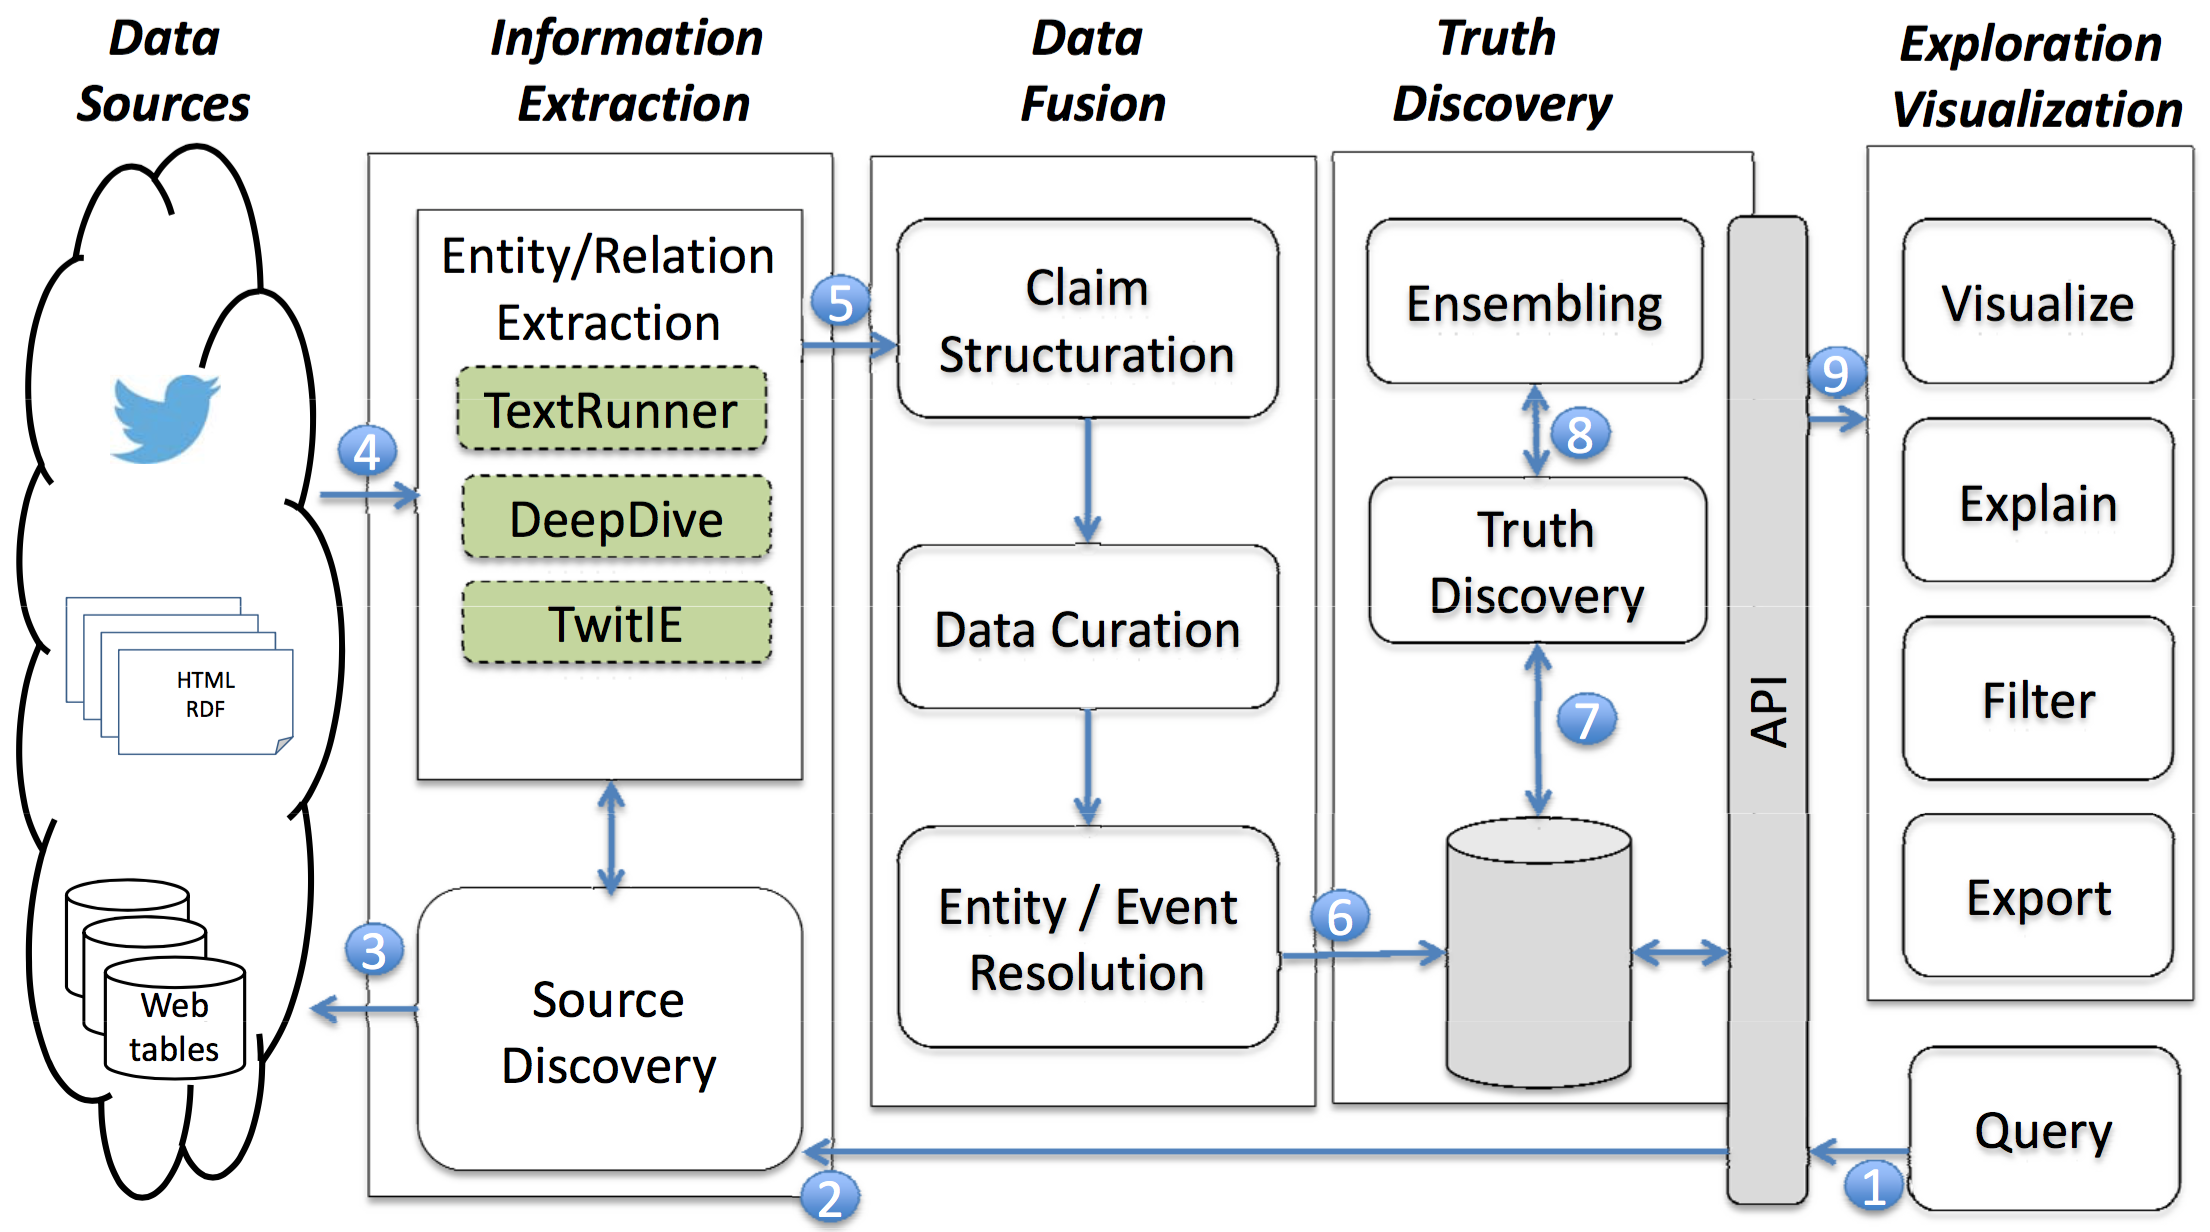
\includegraphics[width=.98\linewidth]{fig1.png}
   \end{center}
\label{archi}\caption{$\VERA$ Architecture }
\end{figure}